\documentclass[11pt]{article}
% Shared LaTeX preamble for Watchdog docs.
\usepackage[margin=1in]{geometry}
\usepackage[T1]{fontenc}
\usepackage{lmodern}
\usepackage{microtype}
\usepackage{graphicx}
\usepackage{xcolor}
\usepackage{hyperref}
\usepackage{booktabs}
\usepackage{longtable}
\usepackage{enumitem}
\usepackage{titlesec}

\hypersetup{
  colorlinks=true,
  linkcolor=blue,
  urlcolor=blue,
  citecolor=blue
}

\setlist[itemize]{noitemsep,topsep=2pt,leftmargin=1.2em}
\setlist[enumerate]{noitemsep,topsep=2pt,leftmargin=1.6em}

\titleformat{\section}{\Large\bfseries}{\thesection}{0.6em}{}
\titleformat{\subsection}{\large\bfseries}{\thesubsection}{0.6em}{}

\newcommand{\watchdog}{Watchdog}
\newcommand{\service}[1]{\texttt{#1}}
\newcommand{\apiendpoint}[1]{\texttt{#1}}

% Diagrams are rendered to ../diagrams/images (relative to docs/latex).
\graphicspath{{../diagrams/images/}}


\title{\watchdog{} --- Design Document (Prototype-Friendly)}
\author{}
\date{March 20, 2026}

\begin{document}
\maketitle

\section{Purpose}
This document captures a concrete, implementable design while keeping enough flexibility to support multiple architecture prototypes.
Once a prototype is selected, this document will be tightened to that specific design.

\section{Selected Target}
The current target is \textbf{Prototype C (log store + async enrichment)} with a critical policy:
\textbf{internal service-to-service APIs use gRPC}.

\section{Service Responsibilities}

\subsection{\service{watcher-service} (Ingestion)}
\begin{itemize}
  \item Accept \apiendpoint{POST /api/v1/ingest} for logs/metrics.
  \item Validate payload shape and reject invalid events early.
  \item Normalize into a common event envelope (kind, source, timestamp, correlation ID).
  \item Forward normalized events downstream (gRPC in Prototype A; broker publish in Prototype B/C).
\end{itemize}

\subsection{\service{core-service} (Orchestration)}
\begin{itemize}
  \item Expose authenticated ticket management endpoints (create/list/get, then update/comment).
  \item Apply rules to decide if an event should open a ticket or update an existing one.
  \item Store tickets in PostgreSQL (database-per-service).
  \item Trigger enrichment for log events and persist enrichment results.
\end{itemize}

\subsection{\service{nlp-service} (Enrichment)}
\begin{itemize}
  \item Expose a gRPC API for text enrichment: \texttt{watchdog.nlp.v1.Analyzer/Analyze}.
  \item The current REST endpoint (\texttt{/api/internal/nlp/analyze}) is legacy and should be deprecated once gRPC is wired end-to-end.
  \item Return category, severity, confidence, and extracted entities.
  \item Evolve from heuristics to model-backed inference without changing the contract.
\end{itemize}

\section{Internal APIs: gRPC First}
\watchdog{} uses gRPC for service-to-service calls to enforce strong typing and compatibility across languages.
Proto definitions live under \texttt{contracts/grpc/}.

\section{Messaging: Kafka}
Kafka is the default message broker.
For Prototype C, the broker carries small pointer and enrichment events; raw payloads live in the log store.

\textbf{Suggested topics (v1):}
\begin{itemize}
  \item \texttt{watchdog.pointer-events.v1}
  \item \texttt{watchdog.enrichment-events.v1}
  \item \texttt{watchdog.dlq.v1}
\end{itemize}

\section{Database + Auth: Supabase}
\textbf{Database:} Supabase Postgres stores tickets and related entities.

\textbf{Auth:} Supabase Auth issues JWTs for operators and service accounts.
\begin{itemize}
  \item Public-facing APIs validate Supabase JWTs.
  \item Local development can validate HS256 tokens using the shared Supabase JWT secret.
  \item Production should validate using the issuer configuration and the provider's published keys/claims policy.
\end{itemize}

\section{Contracts}
\subsection{Event Envelope (Logical)}
All prototypes benefit from a shared logical envelope (even when transported over REST).

\begin{longtable}{@{}p{0.22\linewidth}p{0.16\linewidth}p{0.56\linewidth}@{}}
\toprule
\textbf{Field} & \textbf{Type} & \textbf{Meaning} \\
\midrule
\texttt{event\_id} & string/UUID & Unique ID for idempotency and deduplication \\
\texttt{occurred\_at} & timestamp & When the event happened at the source \\
\texttt{received\_at} & timestamp & When \service{watcher-service} received it \\
\texttt{kind} & enum & \texttt{LOG} or \texttt{METRIC} \\
\texttt{source} & string & Producing system name (payments, auth, etc.) \\
\texttt{correlation\_id} & string & Traces a workflow across services \\
\texttt{payload} & object & Log text or metric name/value and tags \\
\bottomrule
\end{longtable}

\section{Data Model (Ticket)}
\begin{figure}[h]
  \centering
  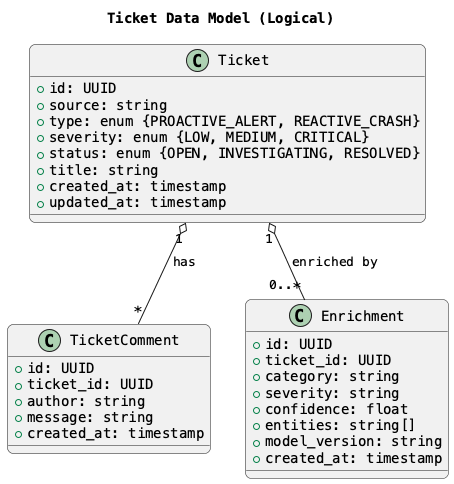
\includegraphics[width=\linewidth]{ticket-data-model.png}
  \caption{Ticket data model (logical)}
\end{figure}

\section{Deployment (Local Development)}
\begin{figure}[h]
  \centering
  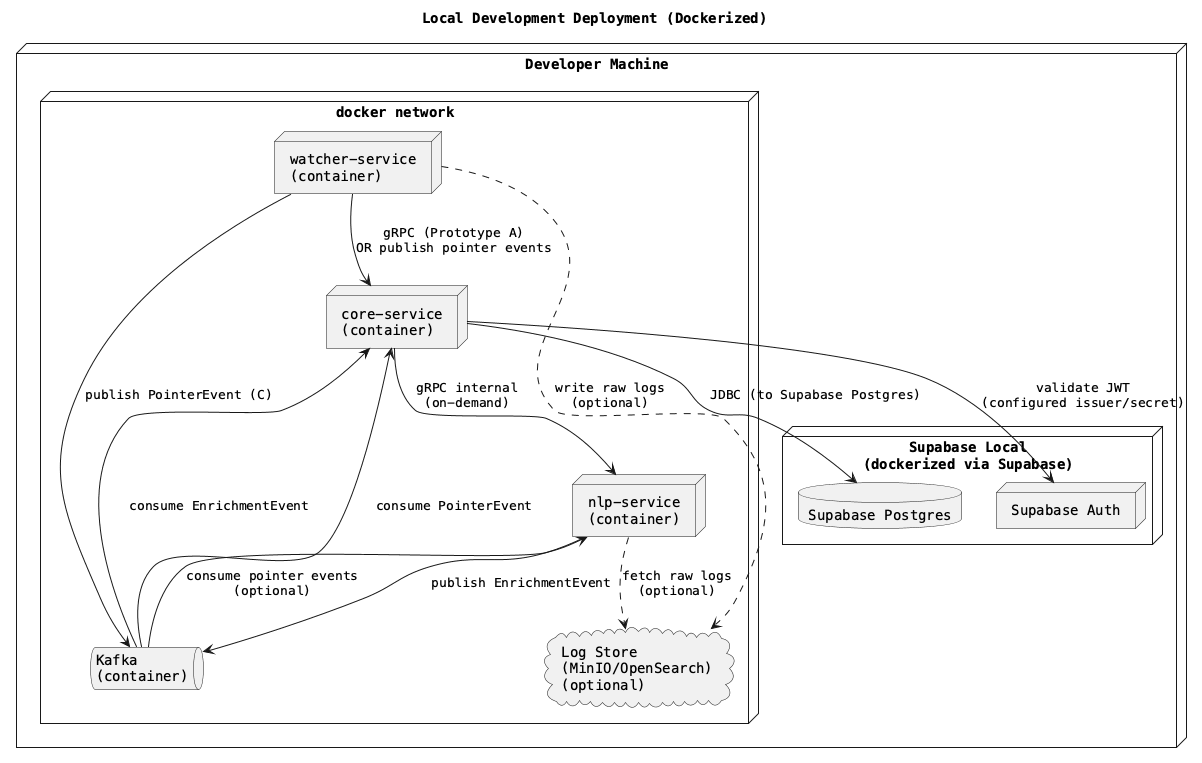
\includegraphics[width=\linewidth]{deployment-local.png}
  \caption{Local docker-compose style deployment}
\end{figure}

\section{Non-Functional Requirements (Initial Targets)}
\begin{itemize}
  \item Reliability: safe retries and idempotency across ingestion paths.
  \item Performance: ingestion remains responsive under bursts (buffering/backpressure).
  \item Security: authenticated management APIs; least-privilege service credentials.
  \item Operability: health checks, structured logs, and basic metrics.
\end{itemize}

\end{document}
